\subsection{Photovoltaic generators} \label{sec:photovoltaic_generators}
The aim of this subsection is to model the \emph{electrical power output} $P_{\mathrm{PV}}$ in $\left( \mathrm W \right)$ of a PV generator based on the previous findings. Since most commercial PV generators consist of PV cells connected in series, only these are going to be covered. Figure \ref{fig:tikz_PVG_circuit_diagram} shows the \emph{electrical equivalent circuit} (EEC) of such a PV generator with a given \emph{number of PV cells} $N_{\mathrm{C}}$ in $\left( 1 \right)$.
\begin{figure}[h!]
	\centering
	

\tikzset{every picture/.style={line width=0.75pt}} %set default line width to 0.75pt        

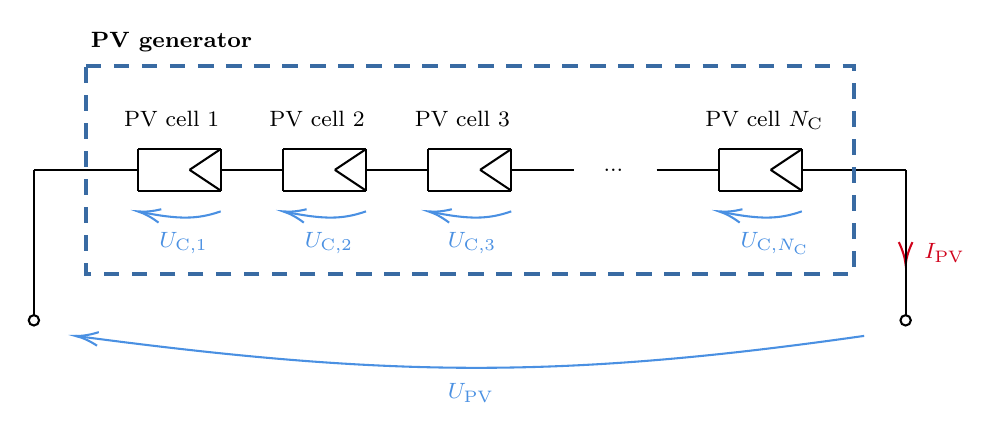
\begin{tikzpicture}[x=0.75pt,y=0.75pt,yscale=-1,xscale=1]
%uncomment if require: \path (0,300); %set diagram left start at 0, and has height of 300

%Straight Lines [id:da607551945482224] 
\draw [color={rgb, 255:red, 208; green, 2; blue, 27 }  ,draw opacity=1 ]   (560,180) -- (560,193.75) ;
\draw [shift={(560,195.75)}, rotate = 270] [color={rgb, 255:red, 208; green, 2; blue, 27 }  ,draw opacity=1 ][line width=0.75]    (10.93,-3.29) .. controls (6.95,-1.4) and (3.31,-0.3) .. (0,0) .. controls (3.31,0.3) and (6.95,1.4) .. (10.93,3.29)   ;
%Straight Lines [id:da39220891738716435] 
\draw    (370,140) -- (370,160) ;
%Straight Lines [id:da26376681003549773] 
\draw    (370,140) -- (355,150) ;
%Straight Lines [id:da7171194033958681] 
\draw    (355,150) -- (370,160) ;
%Straight Lines [id:da7758232590553849] 
\draw    (370,140) -- (330,140) ;
%Straight Lines [id:da23922780724985704] 
\draw    (370,160) -- (330,160) ;
%Straight Lines [id:da8647396746050291] 
\draw    (330,140) -- (330,160) ;
%Shape: Circle [id:dp9465717065223571] 
\draw   (560,220) .. controls (561.38,220) and (562.5,221.12) .. (562.5,222.5) .. controls (562.5,223.88) and (561.38,225) .. (560,225) .. controls (558.62,225) and (557.5,223.88) .. (557.5,222.5) .. controls (557.5,221.12) and (558.62,220) .. (560,220) -- cycle ;
%Straight Lines [id:da8361729954042678] 
\draw    (300,140) -- (300,160) ;
%Straight Lines [id:da8303503310697085] 
\draw    (300,140) -- (285,150) ;
%Straight Lines [id:da6935206293495084] 
\draw    (285,150) -- (300,160) ;
%Straight Lines [id:da4478328338561339] 
\draw    (300,140) -- (260,140) ;
%Straight Lines [id:da6338115192168345] 
\draw    (300,160) -- (260,160) ;
%Straight Lines [id:da4710313866121387] 
\draw    (260,140) -- (260,160) ;
%Straight Lines [id:da04529427678773623] 
\draw    (510,140) -- (510,160) ;
%Straight Lines [id:da12585917694032633] 
\draw    (510,140) -- (495,150) ;
%Straight Lines [id:da5777912998057524] 
\draw    (495,150) -- (510,160) ;
%Straight Lines [id:da8526647582658238] 
\draw    (510,140) -- (470,140) ;
%Straight Lines [id:da18181567227521733] 
\draw    (510,160) -- (470,160) ;
%Straight Lines [id:da08821152259447507] 
\draw    (470,140) -- (470,160) ;
%Straight Lines [id:da004318261204414364] 
\draw    (300,150) -- (330,150) ;
%Straight Lines [id:da415576466861697] 
\draw    (440,150) -- (470,150) ;
%Straight Lines [id:da5030082829613725] 
\draw    (230,140) -- (230,160) ;
%Straight Lines [id:da24153450583970604] 
\draw    (230,140) -- (215,150) ;
%Straight Lines [id:da7169826080141817] 
\draw    (215,150) -- (230,160) ;
%Straight Lines [id:da8893075482646204] 
\draw    (230,140) -- (190,140) ;
%Straight Lines [id:da8414185658377555] 
\draw    (230,160) -- (190,160) ;
%Straight Lines [id:da030501270201809483] 
\draw    (190,140) -- (190,160) ;
%Straight Lines [id:da11000547395248828] 
\draw    (140,150) -- (190,150) ;
%Straight Lines [id:da8573962154803463] 
\draw    (230,150) -- (260,150) ;
%Straight Lines [id:da9793828451968309] 
\draw    (370,150) -- (400,150) ;
%Straight Lines [id:da6281863128480734] 
\draw    (510,150) -- (560,150) ;
%Shape: Rectangle [id:dp583588773515656] 
\draw  [color={rgb, 255:red, 57; green, 107; blue, 163 }  ,draw opacity=1 ][dash pattern={on 5.63pt off 4.5pt}][line width=1.5]  (165,100) -- (535,100) -- (535,200) -- (165,200) -- cycle ;
%Curve Lines [id:da418839437477464] 
\draw [color={rgb, 255:red, 74; green, 144; blue, 226 }  ,draw opacity=1 ]   (230,170) .. controls (218.85,173.88) and (210.04,174) .. (191.73,170.35) ;
\draw [shift={(190,170)}, rotate = 371.59000000000003] [color={rgb, 255:red, 74; green, 144; blue, 226 }  ,draw opacity=1 ][line width=0.75]    (10.93,-3.29) .. controls (6.95,-1.4) and (3.31,-0.3) .. (0,0) .. controls (3.31,0.3) and (6.95,1.4) .. (10.93,3.29)   ;
%Curve Lines [id:da498717897550782] 
\draw [color={rgb, 255:red, 74; green, 144; blue, 226 }  ,draw opacity=1 ]   (300,170) .. controls (288.84,173.88) and (280.04,174) .. (261.73,170.35) ;
\draw [shift={(260,170)}, rotate = 371.59000000000003] [color={rgb, 255:red, 74; green, 144; blue, 226 }  ,draw opacity=1 ][line width=0.75]    (10.93,-3.29) .. controls (6.95,-1.4) and (3.31,-0.3) .. (0,0) .. controls (3.31,0.3) and (6.95,1.4) .. (10.93,3.29)   ;
%Curve Lines [id:da08475302030352005] 
\draw [color={rgb, 255:red, 74; green, 144; blue, 226 }  ,draw opacity=1 ]   (370,170) .. controls (358.85,173.88) and (350.04,174) .. (331.73,170.35) ;
\draw [shift={(330,170)}, rotate = 371.59000000000003] [color={rgb, 255:red, 74; green, 144; blue, 226 }  ,draw opacity=1 ][line width=0.75]    (10.93,-3.29) .. controls (6.95,-1.4) and (3.31,-0.3) .. (0,0) .. controls (3.31,0.3) and (6.95,1.4) .. (10.93,3.29)   ;
%Curve Lines [id:da12741622664998054] 
\draw [color={rgb, 255:red, 74; green, 144; blue, 226 }  ,draw opacity=1 ]   (510,170) .. controls (498.85,173.88) and (490.04,174) .. (471.73,170.35) ;
\draw [shift={(470,170)}, rotate = 371.59000000000003] [color={rgb, 255:red, 74; green, 144; blue, 226 }  ,draw opacity=1 ][line width=0.75]    (10.93,-3.29) .. controls (6.95,-1.4) and (3.31,-0.3) .. (0,0) .. controls (3.31,0.3) and (6.95,1.4) .. (10.93,3.29)   ;
%Straight Lines [id:da46920157249938654] 
\draw    (560,150) -- (560,220) ;
%Shape: Circle [id:dp649544243274581] 
\draw   (140,220) .. controls (141.38,220) and (142.5,221.12) .. (142.5,222.5) .. controls (142.5,223.88) and (141.38,225) .. (140,225) .. controls (138.62,225) and (137.5,223.88) .. (137.5,222.5) .. controls (137.5,221.12) and (138.62,220) .. (140,220) -- cycle ;
%Straight Lines [id:da23605717922255787] 
\draw    (140,150) -- (140,220) ;
%Curve Lines [id:da371666183196145] 
\draw [color={rgb, 255:red, 74; green, 144; blue, 226 }  ,draw opacity=1 ]   (540,230) .. controls (392.5,251) and (310.5,250) .. (160,230) ;
\draw [shift={(160,230)}, rotate = 367.57] [color={rgb, 255:red, 74; green, 144; blue, 226 }  ,draw opacity=1 ][line width=0.75]    (10.93,-3.29) .. controls (6.95,-1.4) and (3.31,-0.3) .. (0,0) .. controls (3.31,0.3) and (6.95,1.4) .. (10.93,3.29)   ;

% Text Node
\draw (182,120) node [anchor=north west][inner sep=0.75pt]  [font=\footnotesize] [align=left] {PV cell $\displaystyle 1$};
% Text Node
\draw (567.5,183.9) node [anchor=north west][inner sep=0.75pt]  [font=\footnotesize,color={rgb, 255:red, 208; green, 2; blue, 27 }  ,opacity=1 ]  {$I_{\mathrm{PV}}$};
% Text Node
\draw (199,178.4) node [anchor=north west][inner sep=0.75pt]  [font=\footnotesize,color={rgb, 255:red, 74; green, 144; blue, 226 }  ,opacity=1 ]  {$U_{\mathrm{C,} 1}$};
% Text Node
\draw (269,178.4) node [anchor=north west][inner sep=0.75pt]  [font=\footnotesize,color={rgb, 255:red, 74; green, 144; blue, 226 }  ,opacity=1 ]  {$U_{\mathrm{C} ,2}$};
% Text Node
\draw (338,178.4) node [anchor=north west][inner sep=0.75pt]  [font=\footnotesize,color={rgb, 255:red, 74; green, 144; blue, 226 }  ,opacity=1 ]  {$U_{\mathrm{C} ,3}$};
% Text Node
\draw (479,178.4) node [anchor=north west][inner sep=0.75pt]  [font=\footnotesize,color={rgb, 255:red, 74; green, 144; blue, 226 }  ,opacity=1 ]  {$U_{\mathrm{C} ,N_{\mathrm{C}}}$};
% Text Node
\draw (252,120) node [anchor=north west][inner sep=0.75pt]  [font=\footnotesize] [align=left] {PV cell $\displaystyle 2$};
% Text Node
\draw (322,120) node [anchor=north west][inner sep=0.75pt]  [font=\footnotesize] [align=left] {PV cell $\displaystyle 3$};
% Text Node
\draw (462,120) node [anchor=north west][inner sep=0.75pt]  [font=\footnotesize] [align=left] {PV cell $\displaystyle N_{\mathrm{C}}$};
% Text Node
\draw (338,251.4) node [anchor=north west][inner sep=0.75pt]  [font=\footnotesize,color={rgb, 255:red, 74; green, 144; blue, 226 }  ,opacity=1 ]  {$U_{\mathrm{PV}}$};
% Text Node
\draw (413,148) node [anchor=north west][inner sep=0.75pt]  [font=\footnotesize] [align=left] {...};
% Text Node
\draw (166,82) node [anchor=north west][inner sep=0.75pt]  [font=\footnotesize] [align=left] {\textbf{PV generator}};


\end{tikzpicture}

	\caption{Electrical equivalent circuit of a photovoltaic generator. It consists of $N_{\mathrm{C}}$ photovoltaic cells connected in series. (Recreated from: \cite{Mertens:2015})}
	\label{fig:tikz_PVG_circuit_diagram}
\end{figure}
As illustrated, $I_{\mathrm{PV}}$ is equal for all PV cells and $U_{\mathrm{PV}}$ is the sum of the \emph{PV cell voltages} $U_{\mathrm{C}}$ in $\left( \mathrm{V} \right)$. It is assumed that all PV cells have the same voltage $U_{\mathrm{C}}$ and therefore $U_{\mathrm{PV}}$ can be written as presented in the equation (\ref{eq:u_pvg_sum_of_pvc}). For the sake of simplicity it is furthermore assumed that the PV generator is installed in a way so that no shadowing occurs during the course of the mission \cite{Prechtl:2006, Mertens:2015}.
	\begin{equation} \label{eq:u_pvg_sum_of_pvc}
	\centering
		U_{\mathrm{PV}} = N_{\mathrm{C}} \, U_{\mathrm{C}}
	\end{equation}

In the next step the PV cells shown in figure \ref{fig:tikz_PVG_circuit_diagram} must be modeled. For this, the simplified standard model\footnote{This model can be derived from the PV cell standard model for $R_{\mathrm{P}} \to \infty$ and $R_{\mathrm{S}} = 0\Omega$.} is used as there are explicit solutions for $U_{\mathrm{C}}$ and $I_{\mathrm{PV}}$. It represents an ideal PV cell without internal losses. An illustration of this model is provided in figure \ref{fig:tikz_PVC_simplified} \cite{Mertens:2015, Wagner:2018}.
\begin{figure}[h!]
	\centering
	

\tikzset{every picture/.style={line width=0.75pt}} %set default line width to 0.75pt        

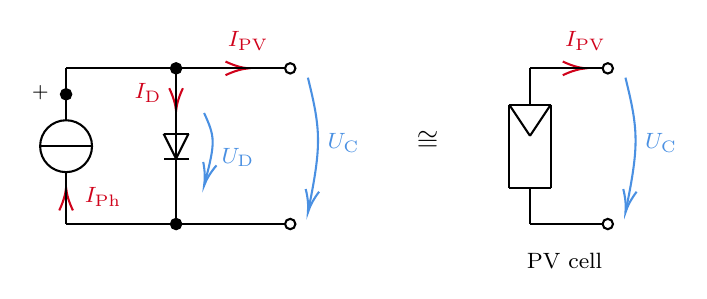
\begin{tikzpicture}[x=0.75pt,y=0.75pt,yscale=-1,xscale=1]
%uncomment if require: \path (0,391); %set diagram left start at 0, and has height of 391

%Straight Lines [id:da9220046892300695] 
\draw [color={rgb, 255:red, 208; green, 2; blue, 27 }  ,draw opacity=1 ]   (259.5,142.5) -- (273.25,142.5) ;
\draw [shift={(275.25,142.5)}, rotate = 180] [color={rgb, 255:red, 208; green, 2; blue, 27 }  ,draw opacity=1 ][line width=0.75]    (10.93,-3.29) .. controls (6.95,-1.4) and (3.31,-0.3) .. (0,0) .. controls (3.31,0.3) and (6.95,1.4) .. (10.93,3.29)   ;
%Straight Lines [id:da9695421868123493] 
\draw [color={rgb, 255:red, 208; green, 2; blue, 27 }  ,draw opacity=1 ]   (422,142.5) -- (435.75,142.5) ;
\draw [shift={(437.75,142.5)}, rotate = 180] [color={rgb, 255:red, 208; green, 2; blue, 27 }  ,draw opacity=1 ][line width=0.75]    (10.93,-3.29) .. controls (6.95,-1.4) and (3.31,-0.3) .. (0,0) .. controls (3.31,0.3) and (6.95,1.4) .. (10.93,3.29)   ;
%Straight Lines [id:da29339333794333666] 
\draw [color={rgb, 255:red, 208; green, 2; blue, 27 }  ,draw opacity=1 ]   (240.5,142.5) -- (240.5,161) ;
\draw [shift={(240.5,163)}, rotate = 270] [color={rgb, 255:red, 208; green, 2; blue, 27 }  ,draw opacity=1 ][line width=0.75]    (10.93,-3.29) .. controls (6.95,-1.4) and (3.31,-0.3) .. (0,0) .. controls (3.31,0.3) and (6.95,1.4) .. (10.93,3.29)   ;
%Straight Lines [id:da5182268392298646] 
\draw [color={rgb, 255:red, 208; green, 2; blue, 27 }  ,draw opacity=1 ]   (187.5,212.5) -- (187.5,202) ;
\draw [shift={(187.5,200)}, rotate = 450] [color={rgb, 255:red, 208; green, 2; blue, 27 }  ,draw opacity=1 ][line width=0.75]    (10.93,-3.29) .. controls (6.95,-1.4) and (3.31,-0.3) .. (0,0) .. controls (3.31,0.3) and (6.95,1.4) .. (10.93,3.29)   ;
%Straight Lines [id:da19579076658988703] 
\draw    (187.5,192.5) -- (187.5,217.5) ;
%Straight Lines [id:da500967170364542] 
\draw    (240.5,142.5) -- (240.5,217.5) ;
%Straight Lines [id:da9693092867247253] 
\draw    (187.5,142.5) -- (187.5,167.5) ;
%Straight Lines [id:da3180920793144646] 
\draw    (240.5,186) -- (234.5,186) ;
%Straight Lines [id:da3231236229149821] 
\draw    (246.5,186) -- (240.5,186) ;
%Straight Lines [id:da20274569848223778] 
\draw    (246.5,174) -- (240.5,174) ;
%Straight Lines [id:da4237476648515044] 
\draw    (240.5,174) -- (234.5,174) ;
%Straight Lines [id:da7091520922682297] 
\draw    (234.5,174) -- (240.5,186) ;
%Straight Lines [id:da8216387087718504] 
\draw    (240.5,186) -- (246.5,174) ;
%Shape: Circle [id:dp46632786849059626] 
\draw   (175,180) .. controls (175,173.1) and (180.6,167.5) .. (187.5,167.5) .. controls (194.4,167.5) and (200,173.1) .. (200,180) .. controls (200,186.9) and (194.4,192.5) .. (187.5,192.5) .. controls (180.6,192.5) and (175,186.9) .. (175,180) -- cycle ;
%Straight Lines [id:da6428722008154575] 
\draw    (175,180) -- (200,180) ;
%Shape: Circle [id:dp9143776877359857] 
\draw  [fill={rgb, 255:red, 0; green, 0; blue, 0 }  ,fill opacity=1 ] (238,217.5) .. controls (238,216.12) and (239.12,215) .. (240.5,215) .. controls (241.88,215) and (243,216.12) .. (243,217.5) .. controls (243,218.88) and (241.88,220) .. (240.5,220) .. controls (239.12,220) and (238,218.88) .. (238,217.5) -- cycle ;
%Shape: Circle [id:dp04116434903611532] 
\draw  [fill={rgb, 255:red, 0; green, 0; blue, 0 }  ,fill opacity=1 ] (185,155) .. controls (185,153.62) and (186.12,152.5) .. (187.5,152.5) .. controls (188.88,152.5) and (190,153.62) .. (190,155) .. controls (190,156.38) and (188.88,157.5) .. (187.5,157.5) .. controls (186.12,157.5) and (185,156.38) .. (185,155) -- cycle ;
%Shape: Circle [id:dp7561083964816784] 
\draw  [fill={rgb, 255:red, 0; green, 0; blue, 0 }  ,fill opacity=1 ] (238,142.5) .. controls (238,141.12) and (239.12,140) .. (240.5,140) .. controls (241.88,140) and (243,141.12) .. (243,142.5) .. controls (243,143.88) and (241.88,145) .. (240.5,145) .. controls (239.12,145) and (238,143.88) .. (238,142.5) -- cycle ;
%Curve Lines [id:da12939293693438314] 
\draw [color={rgb, 255:red, 74; green, 144; blue, 226 }  ,draw opacity=1 ]   (254,164) .. controls (259.33,175.64) and (259.5,177.87) .. (254.48,197.16) ;
\draw [shift={(254,199)}, rotate = 284.68] [color={rgb, 255:red, 74; green, 144; blue, 226 }  ,draw opacity=1 ][line width=0.75]    (10.93,-3.29) .. controls (6.95,-1.4) and (3.31,-0.3) .. (0,0) .. controls (3.31,0.3) and (6.95,1.4) .. (10.93,3.29)   ;
%Straight Lines [id:da820440930056753] 
\draw    (401,160) -- (421,160) ;
%Straight Lines [id:da5978422659023195] 
\draw    (401,160) -- (411,175) ;
%Straight Lines [id:da8646077617642114] 
\draw    (411,175) -- (421,160) ;
%Straight Lines [id:da1683854382748906] 
\draw    (401,160) -- (401,200) ;
%Straight Lines [id:da35944219412656886] 
\draw    (421,160) -- (421,200) ;
%Straight Lines [id:da012841517263090685] 
\draw    (401,200) -- (421,200) ;
%Straight Lines [id:da8937999883743217] 
\draw    (411,200) -- (411,217.5) ;
%Shape: Circle [id:dp39581519495881] 
\draw   (446,142.5) .. controls (446,141.12) and (447.12,140) .. (448.5,140) .. controls (449.88,140) and (451,141.12) .. (451,142.5) .. controls (451,143.88) and (449.88,145) .. (448.5,145) .. controls (447.12,145) and (446,143.88) .. (446,142.5) -- cycle ;
%Shape: Circle [id:dp7404102366707606] 
\draw   (446,217.5) .. controls (446,216.12) and (447.12,215) .. (448.5,215) .. controls (449.88,215) and (451,216.12) .. (451,217.5) .. controls (451,218.88) and (449.88,220) .. (448.5,220) .. controls (447.12,220) and (446,218.88) .. (446,217.5) -- cycle ;
%Straight Lines [id:da16056380159184358] 
\draw    (411,142.5) -- (446,142.5) ;
%Straight Lines [id:da8365114488683654] 
\draw    (411,217.5) -- (446,217.5) ;
%Curve Lines [id:da5511080558248806] 
\draw [color={rgb, 255:red, 74; green, 144; blue, 226 }  ,draw opacity=1 ]   (457,147) .. controls (463.37,172.48) and (463.5,179.71) .. (457.38,210.11) ;
\draw [shift={(457,212)}, rotate = 281.48] [color={rgb, 255:red, 74; green, 144; blue, 226 }  ,draw opacity=1 ][line width=0.75]    (10.93,-3.29) .. controls (6.95,-1.4) and (3.31,-0.3) .. (0,0) .. controls (3.31,0.3) and (6.95,1.4) .. (10.93,3.29)   ;
%Straight Lines [id:da725857721119765] 
\draw    (411,142.5) -- (411,160) ;
%Straight Lines [id:da5740090703572132] 
\draw    (187.5,142.5) -- (240.5,142.5) ;
%Straight Lines [id:da4778393661136311] 
\draw    (187.5,217.5) -- (240.5,217.5) ;
%Shape: Circle [id:dp2917985814178987] 
\draw   (293,142.5) .. controls (293,141.12) and (294.12,140) .. (295.5,140) .. controls (296.88,140) and (298,141.12) .. (298,142.5) .. controls (298,143.88) and (296.88,145) .. (295.5,145) .. controls (294.12,145) and (293,143.88) .. (293,142.5) -- cycle ;
%Shape: Circle [id:dp07126668235633615] 
\draw   (293,217.5) .. controls (293,216.12) and (294.12,215) .. (295.5,215) .. controls (296.88,215) and (298,216.12) .. (298,217.5) .. controls (298,218.88) and (296.88,220) .. (295.5,220) .. controls (294.12,220) and (293,218.88) .. (293,217.5) -- cycle ;
%Curve Lines [id:da8740596681425179] 
\draw [color={rgb, 255:red, 74; green, 144; blue, 226 }  ,draw opacity=1 ]   (304,147) .. controls (310.37,172.48) and (310.5,179.71) .. (304.38,210.11) ;
\draw [shift={(304,212)}, rotate = 281.48] [color={rgb, 255:red, 74; green, 144; blue, 226 }  ,draw opacity=1 ][line width=0.75]    (10.93,-3.29) .. controls (6.95,-1.4) and (3.31,-0.3) .. (0,0) .. controls (3.31,0.3) and (6.95,1.4) .. (10.93,3.29)   ;
%Straight Lines [id:da2745454915751546] 
\draw    (240.5,142.5) -- (293.5,142.5) ;
%Straight Lines [id:da3914094245668047] 
\draw    (240.5,217.5) -- (293.5,217.5) ;

% Text Node
\draw (219,148.4) node [anchor=north west][inner sep=0.75pt]  [font=\footnotesize,color={rgb, 255:red, 208; green, 2; blue, 27 }  ,opacity=1 ]  {$I_{\mathrm{D}}$};
% Text Node
\draw (195,198.4) node [anchor=north west][inner sep=0.75pt]  [font=\footnotesize,color={rgb, 255:red, 208; green, 2; blue, 27 }  ,opacity=1 ]  {$I_{\mathrm{Ph}}$};
% Text Node
\draw (261,179.4) node [anchor=north west][inner sep=0.75pt]  [font=\footnotesize,color={rgb, 255:red, 74; green, 144; blue, 226 }  ,opacity=1 ]  {$U_{\mathrm{D}}$};
% Text Node
\draw (355,171.4) node [anchor=north west][inner sep=0.75pt]  [font=\normalsize]  {$\cong $};
% Text Node
\draw (465,172.4) node [anchor=north west][inner sep=0.75pt]  [font=\footnotesize,color={rgb, 255:red, 74; green, 144; blue, 226 }  ,opacity=1 ]  {$U_{\mathrm{C}}$};
% Text Node
\draw (426.5,123.4) node [anchor=north west][inner sep=0.75pt]  [font=\footnotesize,color={rgb, 255:red, 208; green, 2; blue, 27 }  ,opacity=1 ]  {$I_{\mathrm{PV}}$};
% Text Node
\draw (408,230) node [anchor=north west][inner sep=0.75pt]  [font=\footnotesize] [align=left] {PV cell};
% Text Node
\draw (312,172.4) node [anchor=north west][inner sep=0.75pt]  [font=\footnotesize,color={rgb, 255:red, 74; green, 144; blue, 226 }  ,opacity=1 ]  {$U_{\mathrm{C}}$};
% Text Node
\draw (264,123.4) node [anchor=north west][inner sep=0.75pt]  [font=\footnotesize,color={rgb, 255:red, 208; green, 2; blue, 27 }  ,opacity=1 ]  {$I_{\mathrm{PV}}$};
% Text Node
\draw (169.5,149.4) node [anchor=north west][inner sep=0.75pt]  [font=\scriptsize]  {$+$};


\end{tikzpicture}

	\caption{Simplified standard model of a photovoltaic cell. (Recreated from: \cite{Mertens:2015, Wagner:2018})}
	\label{fig:tikz_PVC_simplified}
\end{figure}

After applying Kirchoff's first and second law to the simplified standard model, considering the equation (\ref{eq:u_pvg_sum_of_pvc}) and taking into account that the PV generator's current-voltage characteristic depends on the PV cell temperature $\vartheta_{\mathrm{C}}$ and the radiation flux $\Phi_{\mathrm{G}}$, it can be modeled with the equations (\ref{eq:i_of_u}) and (\ref{eq:u_of_i}).\footnote{Equation (\ref{eq:u_of_i}) can be derived from equations (\ref{eq:i_of_u}).}
	\begin{equation} \label{eq:i_of_u}
	\centering
		I_{\mathrm{PV}}(U_{\mathrm{PV}}, \vartheta_{\mathrm{C}}, \Phi_{\mathrm{G}}) = I_{\mathrm{Ph}} - \underbrace{I_{\mathrm{S}} \left( \exp \left(\frac{U_{\mathrm{PV}}}{m \, N_{\mathrm{C}} \, U_{\mathrm{T}} } \right) - 1  \right)}_{I_{\mathrm{D}}}
	\end{equation}
	\begin{equation} \label{eq:u_of_i}
	\centering
		U_{\mathrm{PV}}(I_{\mathrm{PV}}, \vartheta_{\mathrm{C}}, \Phi_{\mathrm{G}}) = m \, N_{\mathrm{C}} \, U_{\mathrm{T}} \, \ln \left( \frac{I_{\mathrm{Ph}} - I_{\mathrm{PV}} + I_{\mathrm{S}}}{I_{\mathrm{S}}} \right)
	\end{equation}
The diode's \emph{thermal voltage} $U_{\mathrm{T}} = U_{\mathrm{T}}(\vartheta_{\mathrm{C}})$ in $\left( \mathrm{V} \right)$, with $k_\mathrm{B} = 1,380649 \cdot 10^{-23} \mathrm{WsK^{-1}}$ being the \emph{Bolzmann constant} and $e = 1,602176634\cdot10^{-19} \mathrm{As}$ being the \emph{elementary charge}, can be obtained from the equation (\ref{eq:u_temp}).
	\begin{equation} \label{eq:u_temp}
	\centering
		U_{\mathrm{T}}(\vartheta_{\mathrm{C}}) = \frac{ k_\mathrm{B} \left( \vartheta_{\mathrm{C}} + 273,15^\circ \mathrm{C} \right) }{e} \cdot \frac{\mathrm{1K}}{1^\circ \mathrm{C}}
	\end{equation}
$m$ in $\left( 1 \right)$ is the \emph{ideality factor} with the condition $\{m \in \mathbb{R}^+ \mid 2 \geq m \geq 1 \}$. It is an empirical value that is used to model the PV cells more precisely.\footnote{For $m = 1$, $I_\mathrm{D}$ is Shockley's equation.} The quantities $I_{\mathrm{S}} = I_{\mathrm{S}}(\vartheta_{\mathrm{C}})$ in $\left( \mathrm{A} \right)$ and $I_{\mathrm{Ph}} = I_{\mathrm{Ph}}(\vartheta_{\mathrm{C}}, \Phi_{\mathrm{G}})$ in $\left( \mathrm{A} \right)$ are the diode's \emph{reverse saturation current} and the PV cell's \emph{photocurrent} \cite{Prechtl:2006, Mertens:2015, Tietze:2016, Wagner:2018, Elert:2020}. 

Based on the equation (\ref{eq:i_of_u}), the modeled current-voltage characteristic can be visualized as shown in the figure \ref{fig:tikz/tikz_PVG_curve}, where $I_{\mathrm{SC}}(\vartheta_{\mathrm{C}}, \Phi_{\mathrm{G}})$ in $\left( \mathrm{A} \right)$ and $U_{\mathrm{OC}}(\vartheta_{\mathrm{C}}, \Phi_{\mathrm{G}})$ in $\left( \mathrm{V} \right)$ are the PV generator's \emph{short-circuit current} and \emph{open-circuit voltage}. MPP is the \emph{maximum power point} for which the PV generator provides the greatest electrical power in $\left( \mathrm{W} \right)$, with $U_{\mathrm{MPP}}(\vartheta_{\mathrm{C}}, \Phi_{\mathrm{G}})$ being the voltage and $I_{\mathrm{MPP}}(\vartheta_{\mathrm{C}}, \Phi_{\mathrm{G}})$ being the current at MPP \cite{Prechtl:2006, Mertens:2015, Wagner:2018}:
	\begin{equation} \label{eq:p_mpp}
	\centering
		P_{\mathrm{MPP}}(\vartheta_{\mathrm{C}}, \Phi_{\mathrm{G}}) = U_{\mathrm{MPP}} \, I_{\mathrm{MPP}} \text{.}
	\end{equation}
\begin{figure}[h!]
	\centering
	

\tikzset{every picture/.style={line width=0.75pt}} %set default line width to 0.75pt        

\begin{tikzpicture}[x=0.75pt,y=0.75pt,yscale=-1,xscale=1]
%uncomment if require: \path (0,300); %set diagram left start at 0, and has height of 300

%Image [id:dp8816301757772553] 
\draw (309.25,160) node [xscale=-1] {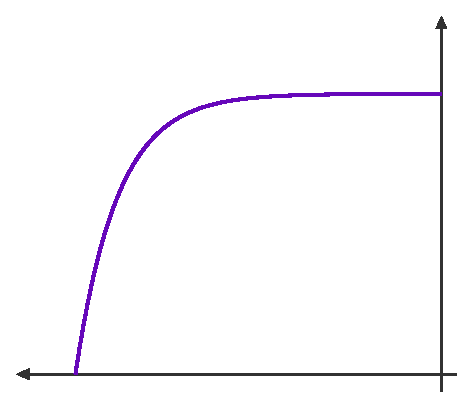
\includegraphics[width=211.13pt,height=180pt]{images/image_PVC_curve}};
%Straight Lines [id:da8531224351110531] 
\draw [color={rgb, 255:red, 155; green, 155; blue, 155 }  ,draw opacity=1 ] [dash pattern={on 4.5pt off 4.5pt}]  (184,113) -- (358,113) ;
%Straight Lines [id:da1728021335997585] 
\draw [color={rgb, 255:red, 155; green, 155; blue, 155 }  ,draw opacity=1 ] [dash pattern={on 4.5pt off 4.5pt}]  (358,113) -- (358,269) ;
%Shape: Circle [id:dp9850794530438081] 
\draw  [fill={rgb, 255:red, 255; green, 255; blue, 255 }  ,fill opacity=1 ] (356,113) .. controls (356,111.9) and (356.9,111) .. (358,111) .. controls (359.1,111) and (360,111.9) .. (360,113) .. controls (360,114.1) and (359.1,115) .. (358,115) .. controls (356.9,115) and (356,114.1) .. (356,113) -- cycle ;

% Text Node
\draw (129,19.4) node [anchor=north west][inner sep=0.75pt]  [font=\footnotesize]  {$I_{\mathrm{PV}}( U_{\mathrm{PV}} ,\vartheta _{\mathrm{C}} ,\Phi _{\mathrm{G}})$};
% Text Node
\draw (456,263.4) node [anchor=north west][inner sep=0.75pt]  [font=\footnotesize]  {$U_{\mathrm{PV}}$};
% Text Node
\draw (278,276.4) node [anchor=north west][inner sep=0.75pt]  [font=\footnotesize]  {$U_{\mathrm{MPP}}( \vartheta _{\mathrm{C}} ,\Phi _{\mathrm{G}})$};
% Text Node
\draw (91,105.4) node [anchor=north west][inner sep=0.75pt]  [font=\footnotesize]  {$I_{\mathrm{MPP}}( \vartheta _{\mathrm{C}} ,\Phi _{\mathrm{G}})$};
% Text Node
\draw (361,96) node [anchor=north west][inner sep=0.75pt]  [font=\footnotesize] [align=left] {MPP};
% Text Node
\draw (370,276.4) node [anchor=north west][inner sep=0.75pt]  [font=\footnotesize]  {$U_{\mathrm{OC}}( \vartheta _{\mathrm{C}} ,\Phi _{\mathrm{G}})$};
% Text Node
\draw (102,83.4) node [anchor=north west][inner sep=0.75pt]  [font=\footnotesize]  {$I_{\mathrm{SC}}( \vartheta _{\mathrm{C}} ,\Phi _{\mathrm{G}})$};
% Text Node
\draw (166,273.4) node [anchor=north west][inner sep=0.75pt]  [font=\footnotesize]  {$0$};


\end{tikzpicture}


	\caption{Modeled current-voltage characteristic of a photovoltaic generator, depending on the radiation flux $\Phi_{\mathrm{G}}$ and the photovoltaic cell temperature $\vartheta_{\mathrm{C}}$. (Recreated from: \cite{Mertens:2015, Wagner:2018})}
	\label{fig:tikz/tikz_PVG_curve}
\end{figure}

The quantity in the simplified standard model that changes with the solar radiation is the photocurrent. It is proportional to the radiation flux $\Phi_{\mathrm{G}}$, with $S = \mathrm{const.}$ in $\left( \mathrm{A}\mathrm{W^{-1}} \right)$ being the \emph{sensitivity} of the PV cell:
	\begin{equation} \label{eq:photo_i}
	\centering
		I_{\mathrm{Ph}}(\vartheta_{\mathrm{STC}}, \Phi_{\mathrm{G}}) = S \, \Phi_{\mathrm{G}} \text{.}
	\end{equation}
From the case $I_{\mathrm{PV}}(0\mathrm{V}, \vartheta_{\mathrm{STC}}, \Phi_{\mathrm{STC}}) = I_\mathrm{SC,STC}$, the sensitivity can be obtained as shown in the equation (\ref{eq:sens}).
	\begin{equation} \label{eq:sens}
	\centering
		 S = \frac{I_\mathrm{SC,STC}}{\Phi_{\mathrm{STC}}}
	\end{equation}
For the \emph{standard test conditions} (STC), listed in the table \ref{tab:table_STC}, $I_\mathrm{SC,STC}$ can be taken directly from the data sheet of a PV generator and $\Phi_{\mathrm{STC}}$ in $\left( \mathrm{W} \right)$ can be calculated using the equation (\ref{eq:radiation_flux}). In this equation, $A_\mathrm{PV}$ can either be measured or taken from a PV generator's data sheet as well.
\begin{table}[h!]
	\centering
	\footnotesize
\begin{tabular}{|l|c|}
	\hline
	\multicolumn{2}{|c|}{\textbf{Standard test conditions for PV generators}} \\
	\hline
 	Total irradiance received by the PV generator & $E_{\mathrm{STC}} = 1000\mathrm{W} \mathrm{m}^{-2}$ \\
	PV cell temperature & $\vartheta_{\mathrm{STC}} = 25^\circ \mathrm{C}$ \\
	Solar spectrum & AM 1,5 \\
	\hline
\end{tabular}
	\caption{Parameters for the standard test conditions of a photovoltaic generator \cite{Mertens:2015}.}
	\label{tab:table_STC}
\end{table}
After substituting equation (\ref{eq:sens}) into equation (\ref{eq:photo_i}) and taking the \emph{temperature coefficient} of the short circuit current $\mathrm{TC}(I_{\mathrm{SC}})$ in $\left( \% ^\circ \mathrm{C}^{-1} \right)$ into account, the photocurrent, depending on the PV cell temperature and the radiation flux, follows to:
	\begin{equation} \label{eq:i_ph_theta_phi}
	\centering
		 I_{\mathrm{Ph}}(\vartheta_{\mathrm{C}}, \Phi_{\mathrm{G}}) = \underbrace{I_{\mathrm{SC,STC}} \, \frac{E_\mathrm{G}}{E_\mathrm{STC}}}_{I_{\mathrm{Ph}}(\vartheta_{\mathrm{STC}}, \Phi_{\mathrm{G}})} \left[ 1 + \frac{\mathrm{TC}(I_{\mathrm{SC}})}{100\%} \left(\vartheta_{\mathrm{C}} - \vartheta_{\mathrm{STC}} \right) \right] \text{.}
	\end{equation}
$\mathrm{TC}(I_{\mathrm{SC}})$ can usually be taken from a PV generator's data sheet.\footnote{Typical $\mathrm{TC}(I_{\mathrm{SC}})$ values for Si-PV cells are around $0,06 \% ^\circ \mathrm{C}^{-1}$.} Because $I_{\mathrm{PV}}(0\mathrm{V}, \vartheta_{\mathrm{C}}, \Phi_{\mathrm{G}}) = I_{\mathrm{SC}}(\vartheta_{\mathrm{C}}, \Phi_{\mathrm{G}})$, $I_{\mathrm{SC}}(\vartheta_{\mathrm{C}}, \Phi_{\mathrm{G}}) = I_{\mathrm{Ph}}(\vartheta_{\mathrm{C}}, \Phi_{\mathrm{G}})$ applies \cite{Mertens:2015, Tietze:2016, Wagner:2018}. 

Now that $I_{\mathrm{Ph}}(\vartheta_{\mathrm{C}}, \Phi_{\mathrm{G}})$ is known, the diode's reverse saturation current can be calculated from the case $I_{\mathrm{PV}}\big(U_{\mathrm{OC}}(\vartheta_{\mathrm{C}}, \Phi_{\mathrm{G}}), \vartheta_{\mathrm{C}}, \Phi_{\mathrm{G}}\big) = 0\mathrm{A}$: 
	\begin{equation} \label{eq:I_S_theta_phi}
	\centering
		I_\mathrm{S}(\vartheta_{\mathrm{C}}) = I_{\mathrm{Ph}}( \vartheta_{\mathrm{C}}, \Phi_{\mathrm{G}}) \left( \exp \left( \frac{U_\mathrm{OC}(\vartheta_{\mathrm{C}}, \Phi_{\mathrm{G}})}{m \, N_\mathrm{C} \, U_\mathrm{T}} \right) - 1 \right)^{-1} \text{.}
	\end{equation}
The open-circuit voltage $U_\mathrm{OC}(\vartheta_{\mathrm{C}}, \Phi_{\mathrm{G}})$ can be derived by subtracting the case $U_{\mathrm{PV}}( 0\mathrm{A}, \vartheta_{\mathrm{C}}, \Phi_{\mathrm{G}})$ from the case $U_{\mathrm{PV}}(0\mathrm{A}, \vartheta_{\mathrm{C}}, \Phi_{\mathrm{STC}})$ while taking the temperature coefficient of the open-circuit voltage $\mathrm{TC}(U_{\mathrm{OC}})$ in $\left( \% ^\circ \mathrm{C}^{-1} \right)$ into account:
	\begin{equation} \label{eq:U_OC_theta_phi}
	\centering
		U_\mathrm{OC}(\vartheta_{\mathrm{C}}, \Phi_{\mathrm{G}}) = U_\mathrm{OC}(\vartheta_{\mathrm{C}},\Phi_\mathrm{STC}) + m \, N_\mathrm{C} \, U_\mathrm{T} \, \ln \left( \frac{I_{\mathrm{Ph}}(\vartheta_{\mathrm{C}}, \Phi_{\mathrm{G}}) + I_{\mathrm{S}}(\vartheta_{\mathrm{C}})}{I_\mathrm{Ph}(\vartheta_{\mathrm{C}},\Phi_\mathrm{STC}) + I_{\mathrm{S}}( \vartheta_{\mathrm{C}})} \right) \text{,}
	\end{equation}
where $U_\mathrm{OC}(\vartheta_{\mathrm{C}},\Phi_\mathrm{STC})$ is the temperature dependent open-circuit voltage for the radiation flux $\Phi_\mathrm{STC}$ at STC: 
	\begin{equation} \label{eq:U_OC_phi_STC}
	\centering
		U_\mathrm{OC}(\vartheta_{\mathrm{C}},\Phi_\mathrm{STC}) = U_\mathrm{OC,STC} \left[ 1 + \frac{\mathrm{TC}(U_{\mathrm{OC}})}{100\%} \left(\vartheta_{\mathrm{C}} - \vartheta_{\mathrm{STC}} \right) \right] \text{.}
	\end{equation}
In addition to $\mathrm{TC}(I_{\mathrm{SC}})$, $\mathrm{TC}(U_{\mathrm{OC}})$ can also be taken from a PV generators data sheet.\footnote{Typical $\mathrm{TC}(U_{\mathrm{OC}})$ values for Si-PV cells are around $-0,40 \% ^\circ \mathrm{C}^{-1}$.} Equation (\ref{eq:U_OC_theta_phi}) is only valid because the reverse saturation current $I_\mathrm{S}(\vartheta_{\mathrm{C}})$ does not depend on the radiation flux \cite{Mertens:2015, Tietze:2016, Hering:2017, Wagner:2018}. 

Since the equations (\ref{eq:I_S_theta_phi}) and (\ref{eq:U_OC_theta_phi}) are in a non-linear relationship to one another, the Newton-Raphson method must be used to approximate them numerically (see appendix \ref{sec:newton_raphson_method}). For this, the functions $f_1(\mathrm{\mathbf{x}}_R)$ and $f_2(\mathrm{\mathbf{x}}_R)$ are introduced below. In the equation (\ref{eq:f_1}) an exponential function is used instead of a logarthmic function, since some numerical approximation algorithms do not converge for logarithmic functions.
	\begin{equation} \label{eq:f_1}
	\centering
		\begin{split}
		f_1(\mathrm{\mathbf{x}}_R) = \exp \left( \frac{U_\mathrm{OC}(\vartheta_{\mathrm{C}}, \Phi_{\mathrm{G}}) - U_\mathrm{OC}(\vartheta_{\mathrm{C}},\Phi_\mathrm{STC})}{m \, N_\mathrm{C} \, U_\mathrm{T}} \right) \\ - \frac{I_{\mathrm{Ph}}(\vartheta_{\mathrm{C}}, \Phi_{\mathrm{G}}) + I_{\mathrm{S}}(\vartheta_{\mathrm{C}})}{I_\mathrm{Ph}(\vartheta_{\mathrm{C}},\Phi_\mathrm{STC}) + I_{\mathrm{S}}(\vartheta_{\mathrm{C}})} = 0
		\end{split}
	\end{equation}
	\begin{equation} \label{eq:f_2}
	\centering
		f_2(\mathrm{\mathbf{x}}_R) = I_\mathrm{S}(\vartheta_{\mathrm{C}}) - I_\mathrm{Ph}(\vartheta_{\mathrm{C}}, \Phi_{\mathrm{G}}) \left(\exp \left(\frac{U_\mathrm{OC}(\vartheta_{\mathrm{C}}, \Phi_{\mathrm{G}})}{m \, N_\mathrm{C} \, U_\mathrm{T}} \right) - 1 \right)^{-1} = 0\mathrm{A}
	\end{equation}
The vector $\mathrm{\mathbf{x}}_R$, shown in the equation (\ref{eq:x_r_vector}), contains the zero crossings of the functions $f_1(\mathrm{\mathbf{x}}_R)$ and $f_2(\mathrm{\mathbf{x}}_R)$. 
	\begin{equation} \label{eq:x_r_vector}
	\centering
		\mathrm{\mathbf{x}}_R = \Big( I_\mathrm{S}(\vartheta_{\mathrm{C}}), U_\mathrm{OC}(\vartheta_{\mathrm{C}}, \Phi_{\mathrm{G}}) \Big)^{\mathrm T}
	\end{equation}
Furthermore, the vector $\mathrm{\mathbf{f}}(\mathrm{\mathbf{x}}_R) = \mathbf{0}$, which contains the functions from the equations (\ref{eq:f_1}) and (\ref{eq:f_2}), must be introduced for the Newton-Raphson method:
	\begin{equation} \label{eq:f_vector}
	\centering
		\mathrm{\mathbf{f}}(\mathrm{\mathbf{x}}_R) = 
  			\Big( f_{1}(\mathrm{\mathbf{x}}_R), f_{2}(\mathrm{\mathbf{x}}_R) \Big)^{\mathrm T} = \mathrm{\mathbf{0}} \text{.}
	\end{equation}
With the help of the Jacobian matrix $\mathrm{\mathbf{J}} = \partial \mathrm{\mathbf{f}}(\mathrm{\mathbf{x}}) / \partial \mathrm{\mathbf{x}}$ for $\mathrm{\mathbf{x}} = \mathrm{\mathbf{x}}_R$, the $\left(n + 1\right)$\textsuperscript{th} approximation with $n \in \mathbb{N}$ can be determined as follows:
	\begin{equation} \label{eq:vect_U_I_approx}
	\centering
		\mathrm{\mathbf{x}}_{R, n + 1} = \mathrm{\mathbf{x}}_{R,n} 	- \mathrm{\mathbf{J}}^{-1}(\mathrm{\mathbf{x}}_{R,n}) \, \mathrm{\mathbf{f}}(\mathrm{\mathbf{x}}_{R,n}) \text{,}
	\end{equation}
	\begin{equation} \label{eq:jacobian_for_PVG}
	\centering
		\mathrm{\mathbf{J}} =  
 		\begin{pmatrix}
  			\dfrac{\partial f_1\big( I_\mathrm{S}(\vartheta_{\mathrm{C}}), U_\mathrm{OC}(\vartheta_{\mathrm{C}},\Phi_{\mathrm{G}}) \big)}{\partial I_\mathrm{S}(\vartheta_{\mathrm{C}})}  & \dfrac{\partial  f_1\big( I_\mathrm{S}(\vartheta_{\mathrm{C}}), U_\mathrm{OC}(\vartheta_{\mathrm{C}},\Phi_{\mathrm{G}}) \big)}{\partial U_\mathrm{OC}(\vartheta_{\mathrm{C}},\Phi_{\mathrm{G}})} \\
			\dfrac{\partial f_2\big( I_\mathrm{S}(\vartheta_{\mathrm{C}}), U_\mathrm{OC}(\vartheta_{\mathrm{C}},\Phi_{\mathrm{G}}) \big)}{\partial I_\mathrm{S}(\vartheta_{\mathrm{C}})} & \dfrac{\partial f_2\big( I_\mathrm{S}(\vartheta_{\mathrm{C}}), U_\mathrm{OC}(\vartheta_{\mathrm{C}},\Phi_{\mathrm{G}}) \big)}{\partial U_\mathrm{OC}(\vartheta_{\mathrm{C}},\Phi_{\mathrm{G}})} 
 		\end{pmatrix} \text{.}
 	\end{equation}
Starting values for the Newton-Raphson method can be obtained from the expressions in the equation (\ref{eq:U_OC_I_S_zero}), if it is accepted that the diode's reverse saturation current $I_{\mathrm{S}}$ is small compared to the photocurrent $I_{\mathrm{Ph}}$, so that $I_{\mathrm{S}} + I_{\mathrm{Ph}} \approx I_{\mathrm{Ph}}$ applies.\footnote{These expressions can be derived from the equations (\ref{eq:U_OC_theta_phi}) and (\ref{eq:I_S_theta_phi}).}
	\begin{equation} \label{eq:U_OC_I_S_zero}
	\centering
		\begin{gathered}
		 U_{\mathrm{OC,0}}(\vartheta_{\mathrm{C}}, \Phi_{\mathrm{G}}) = U_\mathrm{OC}(\vartheta_{\mathrm{C}},\Phi_\mathrm{STC}) + m \, N_\mathrm{C} \, U_\mathrm{T} \, \ln \left( \frac{I_\mathrm{Ph}(\vartheta_{\mathrm{C}}, \Phi_{\mathrm{G}})}{I_\mathrm{Ph}(\vartheta_{\mathrm{C}},\Phi_\mathrm{STC})} \right)\text{,} \\
		 I_\mathrm{S,0}(\vartheta_{\mathrm{C}}) = I_{\mathrm{Ph}}(\vartheta_{\mathrm{C}}, \Phi_{\mathrm{G}}) \, \exp \left( - \frac{U_\mathrm{OC,0}(\vartheta_{\mathrm{C}}, \Phi_{\mathrm{G}})}{m \, N_\mathrm{C} \, U_\mathrm{T}} \right)\text{,} \\ \text{for } I_\mathrm{S} \ll I_\mathrm{Ph}
		 \end{gathered}
	\end{equation}
With these, the starting vector $\mathrm{\mathbf{x}}_{R,0} = \big( I_\mathrm{S,0}(\vartheta_{\mathrm{C}}), U_\mathrm{OC,0}(\vartheta_{\mathrm{C}}, \Phi_{\mathrm{G}}) \big)^{\mathrm T}$ for the first iteration can be obtained. Finally, it has to mentioned that the functions $f_1(\mathrm{\mathbf{x}}_R)$ and $f_2(\mathrm{\mathbf{x}}_R)$ are continuously differentiable for the required number of iteration steps $n + 1$. This is a requirement for the Newton-Raphson method \cite{Schwarz:2011, Rudolf:2014, Taschner:2014, Mertens:2015, Wagner:2018, Kugi:2021}.

The PV cell temperature $\vartheta_{\mathrm{C}}$, depending on the irradiance $E_{\mathrm{G}}$ and the \emph{ambient temperature} $\vartheta_{\mathrm{A}}$ in $\left( ^\circ \mathrm{C} \right)$, with the \emph{nominal operating cell temperature}\footnote{Typical $\mathrm{NOCT}$ values for c-Si-PV generators are around $45$ to $50^\circ \mathrm{C}$.} $\mathrm{NOCT}$ in $\left( ^\circ \mathrm{C} \right)$ and the conditions under which it is measured, $\vartheta_{\mathrm{A,NOCT}}$ in $\left( ^\circ \mathrm{C} \right)$ and $E_{\mathrm{NOCT}}$ in $\left( \mathrm{W} \mathrm{m}^{-2} \right)$, can be approximated by assuming that the increase of $\vartheta_{\mathrm{C}}$, compared to the ambient temperature $\vartheta_{\mathrm{A}}$, is proportional to $E_{\mathrm{G}}$:
	\begin{equation} \label{eq:cell_temp}
	\centering
		\vartheta_{\mathrm{C}} \approx \vartheta_{\mathrm{A}} + \left(\mathrm{NOCT} - \vartheta_{\mathrm{A,NOCT}}\right) \frac{E_{\mathrm{G}}}{E_{\mathrm{NOCT}}} \text{.}
	\end{equation}
The paramateres under which the $\mathrm{NOCT}$ is measured are provided by the table \ref{tab:table_NOCT} and the $\mathrm{NOCT}$ is usually listed in the data sheet of a PV generator \cite{Mertens:2015}.
\begin{table}[h!]
	\centering
	\footnotesize
\begin{tabular}{|l|c|}
	\hline
	\multicolumn{2}{|c|}{\textbf{Conditions for NOCT measurement}} \\
	\hline
 	Total irradiance received by the PV generator & $E_{\mathrm{NOCT}} = 800\mathrm{W} \mathrm{m}^{-2}$ \\
	Ambient temperature & $\vartheta_{\mathrm{A, NOCT}} = 20^\circ \mathrm{C}$ \\
	Wind speed & $v_{\mathrm W} = 1 \mathrm{m} \mathrm{s}^{-1}$  \\
	\hline
\end{tabular}
	\caption{Conditions under which the NOCT is measured \cite{Mertens:2015}.}
	\label{tab:table_NOCT}
\end{table}

Ambient temperatures $\vartheta_{\mathrm{A}}$ for different locations on Earth can be obtained from climate charts. For example, figure \ref{fig:temp_vienna} presents monthly averages for the ambient temperature in $\left( ^\circ \mathrm{C} \right)$ and precipitation in $\left( \mathrm{mm} \right)$ collected by the Global Historical Climatology Network for the Hohe Warte in Vienna, Austria, between 1997 and 2016. Below the chart, the percentage of missing data regarding the months of the year is presented \cite{Zepner:2020}.
\begin{figure}[h!]
	\centering
  	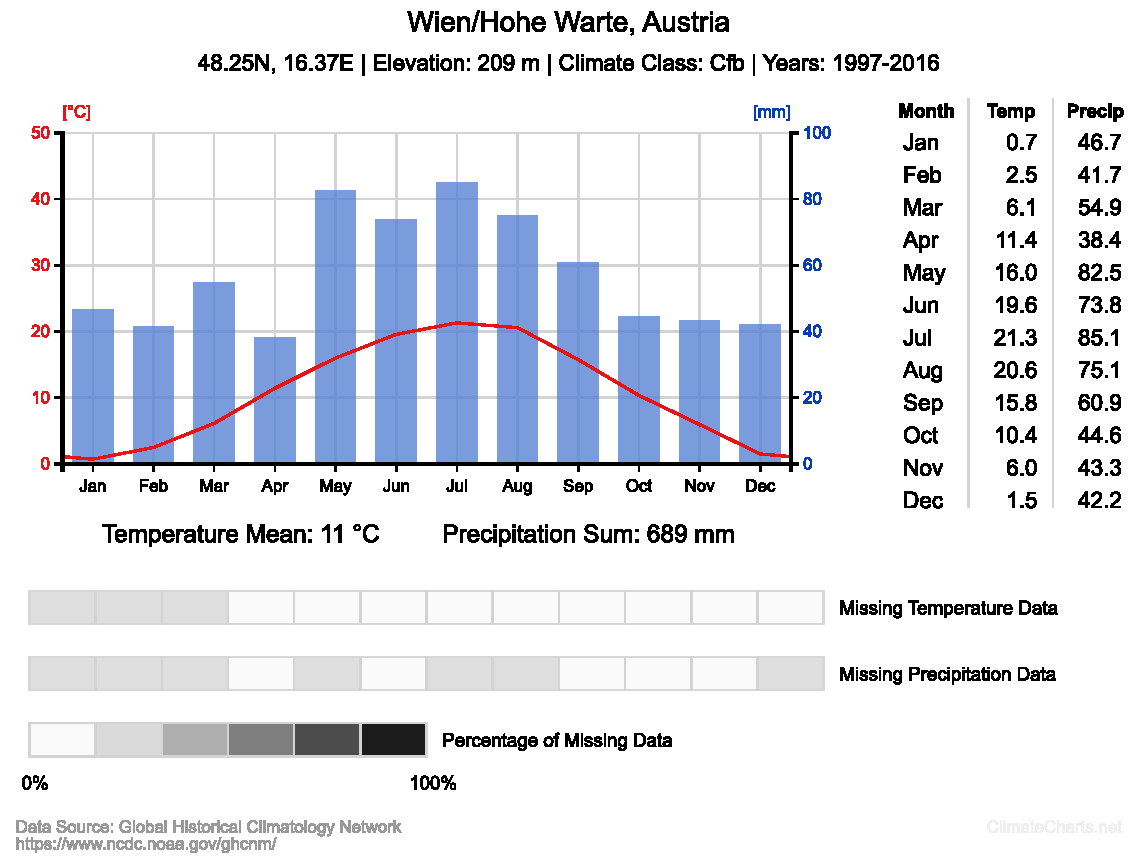
\includegraphics[width = 0.96\textwidth]{temp_maps/temp_vienna}
  	\caption{Monthly averages of temperature and precipitation data for the Hohe Warte in Vienna, Austria. (Image credit: \cite{Zepner:2020})}
	\label{fig:temp_vienna}
\end{figure}

Building on the previous findings, the electrical power output of a PV generator can be calculted by using one of the following equations:
	\begin{equation} \label{eq:p_pv_i}
	\centering
		P_{\mathrm{PV}}(I_{\mathrm{PV}}, \vartheta_{\mathrm{C}}, \Phi_{\mathrm{G}}) = m \, N_{\mathrm{C}} \, U_{\mathrm{T}} \, I_{\mathrm{PV}} \, \ln \left( \frac{I_{\mathrm{Ph}} - I_{\mathrm{PV}} + I_{\mathrm{S}}}{I_{\mathrm{S}}} \right) \text{,}
	\end{equation}
	\begin{equation} \label{eq:p_pv_u}
	\centering
		 P_{\mathrm{PV}}(U_{\mathrm{PV}}, \vartheta_{\mathrm{C}}, \Phi_{\mathrm{G}}) = U_{\mathrm{PV}} \left[ I_{\mathrm{Ph}} - I_{\mathrm{S}} \left( \exp \left(\frac{U_{\mathrm{PV}}}{m \, N_{\mathrm{C}} \, U_{\mathrm{T}} } \right) - 1  \right) \right] \text{.}
	\end{equation}
Typically, $P_{\mathrm{PV}}$ is plotted as a function of $U_{\mathrm{PV}}$, which results in a curve as shown in the figure \ref{fig:tikz_PVG_power_curve} \cite{Prechtl:2006, Mertens:2015, Wagner:2018}.
\begin{figure}[h!]
	\centering
	

\tikzset{every picture/.style={line width=0.75pt}} %set default line width to 0.75pt        

\begin{tikzpicture}[x=0.75pt,y=0.75pt,yscale=-1,xscale=1]
%uncomment if require: \path (0,425); %set diagram left start at 0, and has height of 425

%Image [id:dp09113935256135308] 
\draw (346,215.5) node  {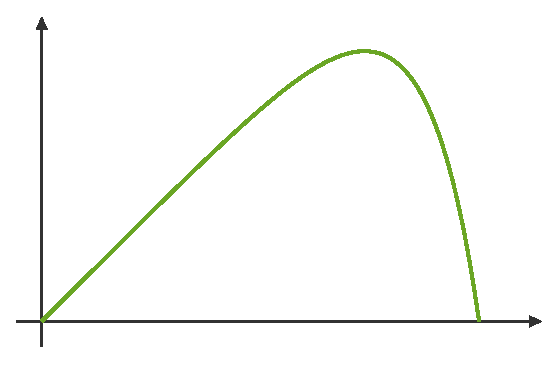
\includegraphics[width=252pt,height=158.25pt]{image_PVG_power_curve}};
%Straight Lines [id:da17852705755040943] 
\draw [color={rgb, 255:red, 155; green, 155; blue, 155 }  ,draw opacity=1 ] [dash pattern={on 4.5pt off 4.5pt}]  (199,132) -- (386,132) ;
%Straight Lines [id:da5125910827691256] 
\draw [color={rgb, 255:red, 155; green, 155; blue, 155 }  ,draw opacity=1 ] [dash pattern={on 4.5pt off 4.5pt}]  (401,138) -- (401,304) ;
%Shape: Circle [id:dp819738962444466] 
\draw  [fill={rgb, 255:red, 255; green, 255; blue, 255 }  ,fill opacity=1 ] (399,132) .. controls (399,130.9) and (399.9,130) .. (401,130) .. controls (402.1,130) and (403,130.9) .. (403,132) .. controls (403,133.1) and (402.1,134) .. (401,134) .. controls (399.9,134) and (399,133.1) .. (399,132) -- cycle ;

% Text Node
\draw (103,123.4) node [anchor=north west][inner sep=0.75pt]  [font=\footnotesize]  {$P_{\mathrm{MPP}}( \vartheta _{\mathrm{C}} ,\Phi _{\mathrm{G}})$};
% Text Node
\draw (334.71,308.4) node [anchor=north west][inner sep=0.75pt]  [font=\footnotesize]  {$U_{\mathrm{MPP}}( \vartheta _{\mathrm{C}} ,\Phi _{\mathrm{G}})$};
% Text Node
\draw (520,298.4) node [anchor=north west][inner sep=0.75pt]  [font=\footnotesize]  {$U_{\mathrm{PV}}$};
% Text Node
\draw (139,89.4) node [anchor=north west][inner sep=0.75pt]  [font=\footnotesize]  {$P_{\mathrm{PV}}( U_{\mathrm{PV}} ,\vartheta _{\mathrm{C}} ,\Phi _{\mathrm{G}})$};
% Text Node
\draw (384.5,112) node [anchor=north west][inner sep=0.75pt]  [font=\footnotesize] [align=left] {MPP};
% Text Node
\draw (427.86,308.4) node [anchor=north west][inner sep=0.75pt]  [font=\footnotesize]  {$U_{\mathrm{OC}}( \vartheta _{\mathrm{C}} ,\Phi _{\mathrm{G}})$};
% Text Node
\draw (180,308.4) node [anchor=north west][inner sep=0.75pt]  [font=\footnotesize]  {$0$};


\end{tikzpicture}

	\caption{Electrical power output of a photovoltaic generator as a function of $U_{\mathrm{PV}}$. It is further dependent on the photovoltaic cell temperature $\vartheta_{\mathrm{C}}$ and the radiation flux $\Phi_{\mathrm{G}}$. (Recreated from: \cite{Mertens:2015})}
	\label{fig:tikz_PVG_power_curve}
\end{figure}